\newpage
\chapter{Isomap}
\subsubsection{Eindimensionales Signal}
\begin{figure}[h]
	\centering
	\subfloat[Ausrei�er-Typ Signal Drift\label{img:dailyDriftIso}]{
		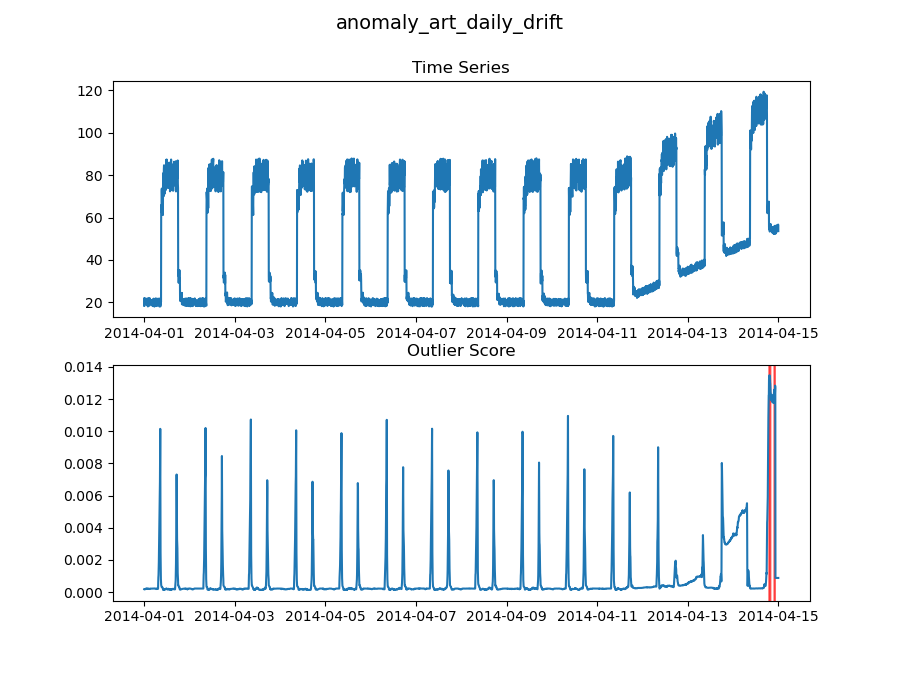
\includegraphics[width=0.5\textwidth]{fig/resultsIsoMap/anomaly_art_daily_drift}}
	\subfloat[Ausrei�er-Typ Zunahme an Rauschen\label{img:increaseNoiseIso}]{
		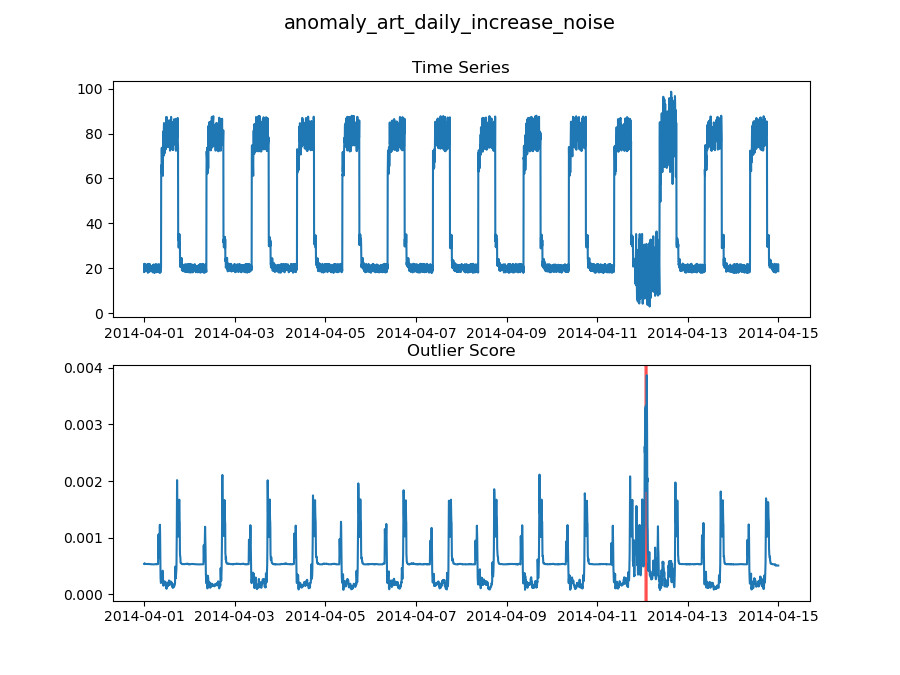
\includegraphics[width=0.5\textwidth]{fig/resultsIsoMap/anomaly_art_daily_increase_noise}}
	\qquad
	\subfloat[Ausrei�er-Typ Einzelne Peaks\label{img:dailyPeaksIso}]{
		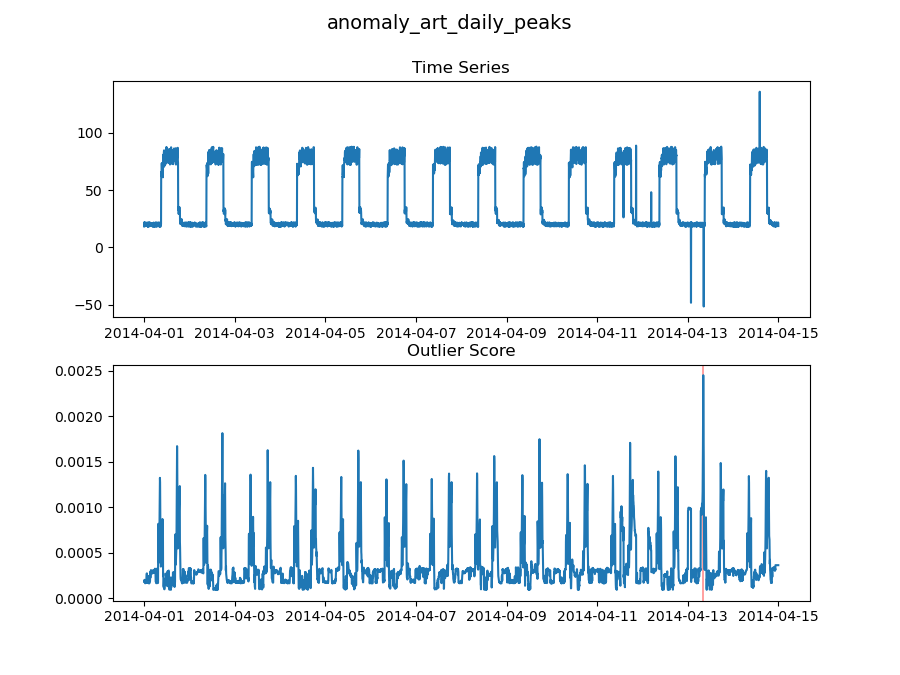
\includegraphics[width=0.5\textwidth]{fig/resultsIsoMap/anomaly_art_daily_peaks}}
	\subfloat[Ausrei�er-Typ Frequenz�nderung\label{img:sequenceChangeIso}]{
		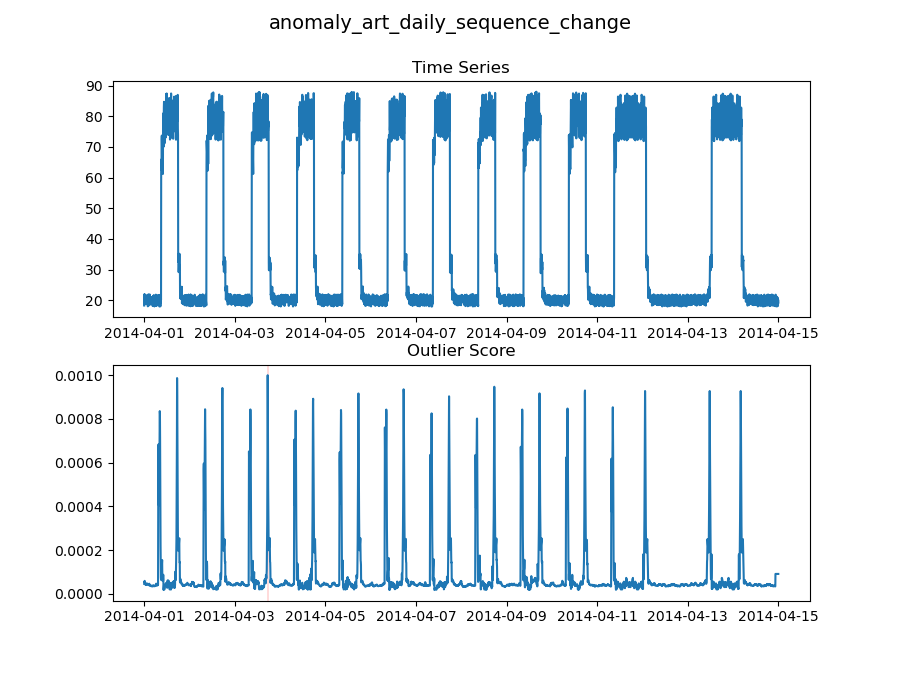
\includegraphics[width=0.5\textwidth]{fig/resultsIsoMap/anomaly_art_daily_sequence_change}}
	\qquad
\end{figure}
\begin{figure}\ContinuedFloat
	\subfloat[Ausrei�er-Typ Kontinuierliche Zunahme der Amplitude\label{img:ampRiseIso}]{
		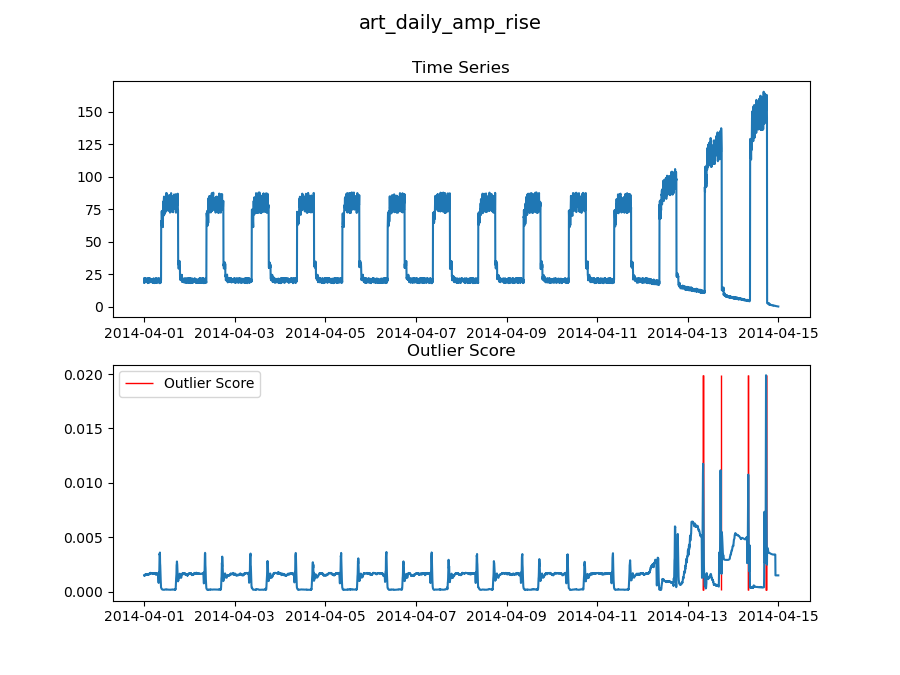
\includegraphics[width=0.5\textwidth]{fig/resultsIsoMap/art_daily_amp_rise}}
	\subfloat[Ausrei�er-Typ Zyklus-Aussetzer\label{img:flatmiddleIso}]{
		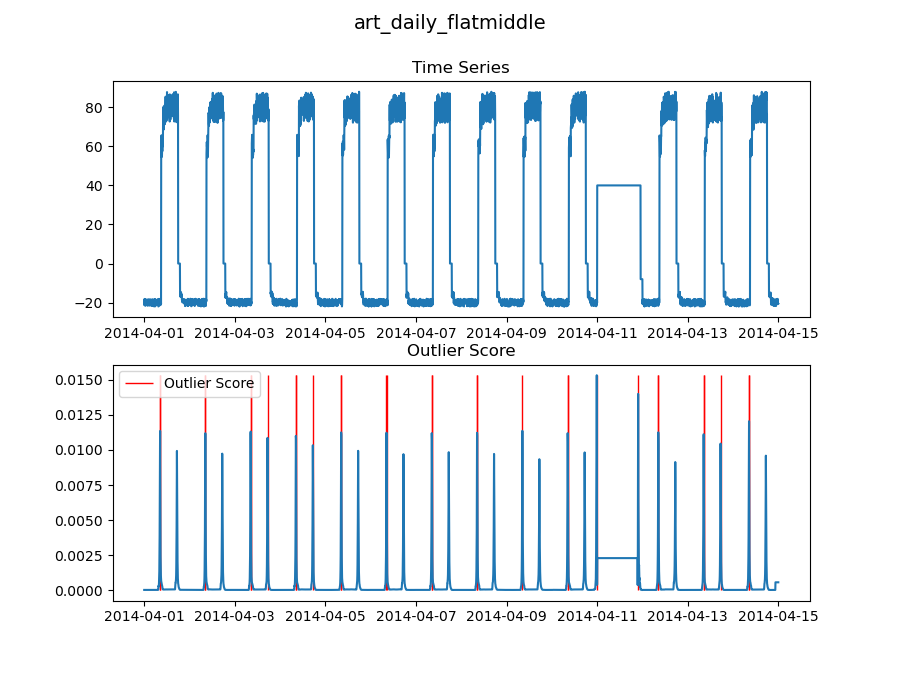
\includegraphics[width=0.5\textwidth]{fig/resultsIsoMap/art_daily_flatmiddle}}
	\qquad
	\subfloat[Ausrei�er-Typ Zyklus mit geringerer Amplitude\label{img:jumpsdownIso}]{
		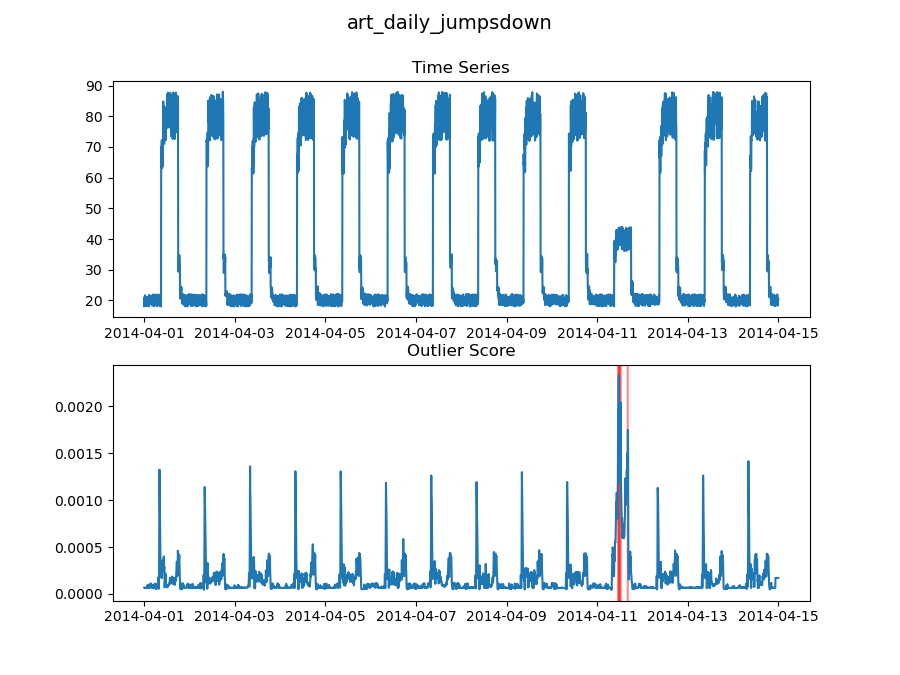
\includegraphics[width=0.5\textwidth]{fig/resultsIsoMap/art_daily_jumpsdown}}
	\subfloat[Ausrei�er-Typ Zyklus mit h�herer Amplitude\label{img:jumpsupIso}]{
		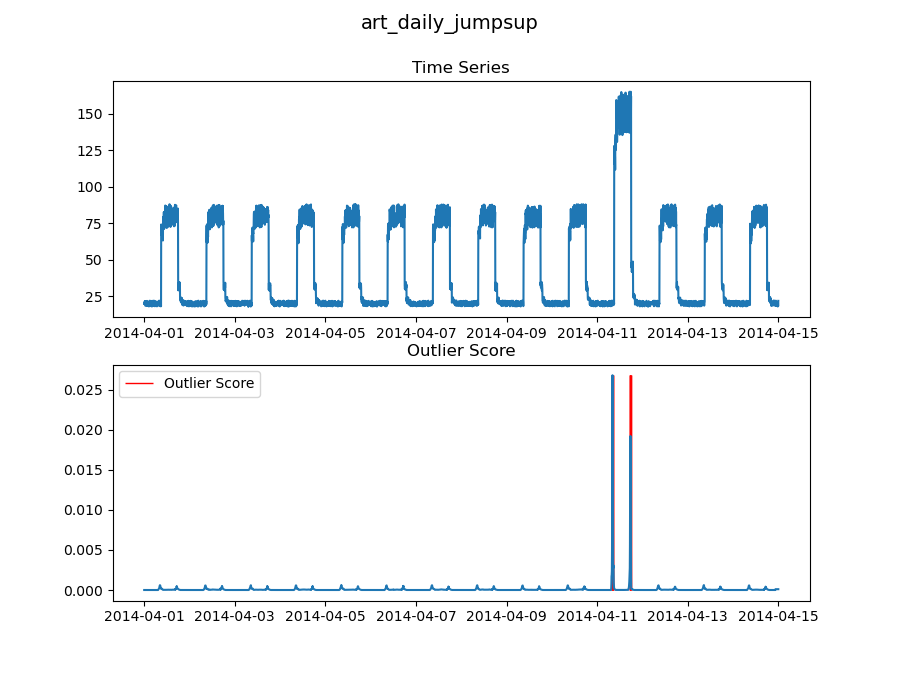
\includegraphics[width=0.5\textwidth]{fig/resultsIsoMap/art_daily_jumpsup}}
	\qquad
	\subfloat[Ausrei�er-Typ Signal-Aussetzer\label{img:nojumpIso}]{
		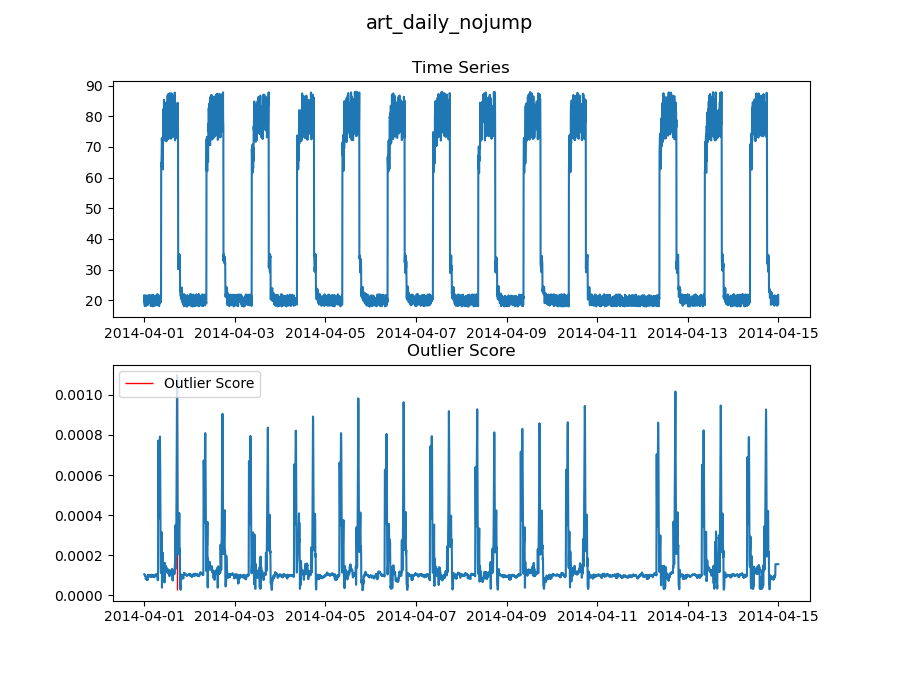
\includegraphics[width=0.5\textwidth]{fig/resultsIsoMap/art_daily_nojump}}
\end{figure}






\newpage
\chapter{Percolation}
\subsubsection{Eindimensionales Signal}
\label{app-perc}
\begin{figure}[h]
	\centering
	\subfloat[Ausrei�er-Typ Signal Drift\label{img:dailyDriftPerc}]{
		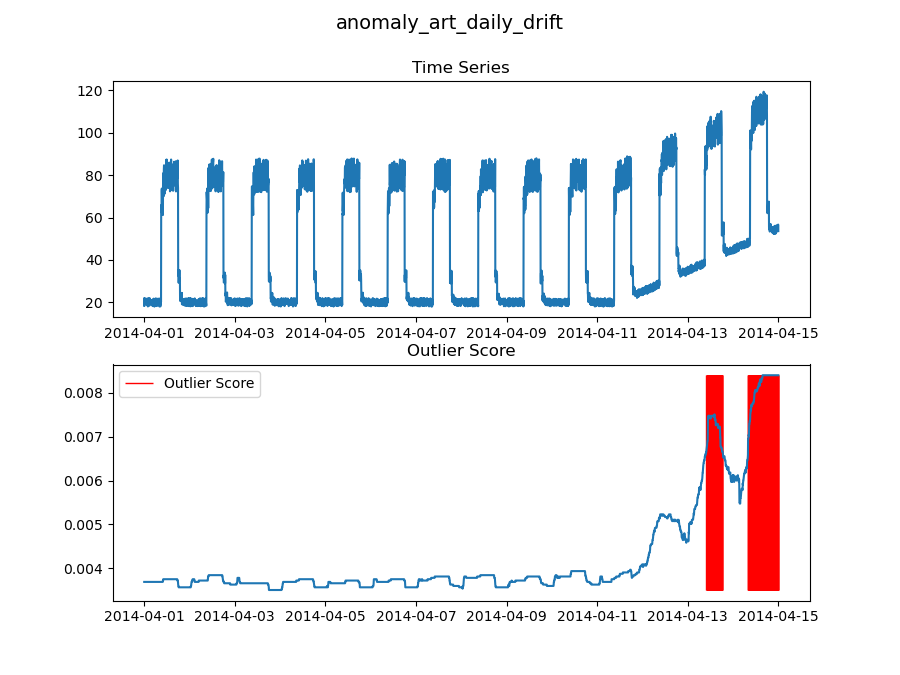
\includegraphics[width=0.5\textwidth]{fig/resultsPercolation/anomaly_art_daily_drift}}
	\subfloat[Ausrei�er-Typ Zunahme an Rauschen\label{img:increaseNoisePerc}]{
		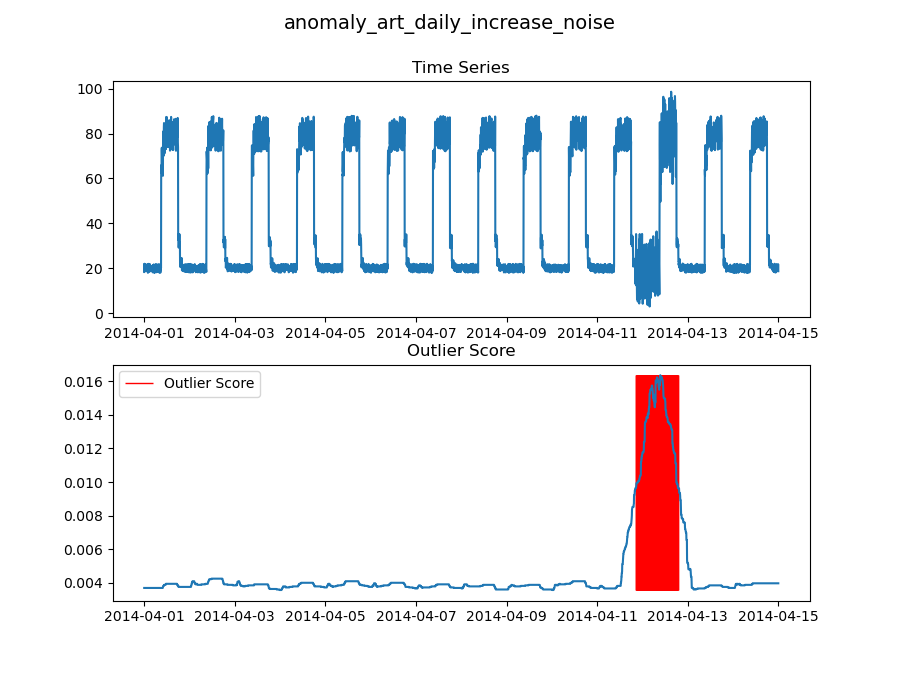
\includegraphics[width=0.5\textwidth]{fig/resultsPercolation/anomaly_art_daily_increase_noise}}
	\qquad
	\subfloat[Ausrei�er-Typ Einzelne Peaks\label{img:dailyPeaksPerc}]{
		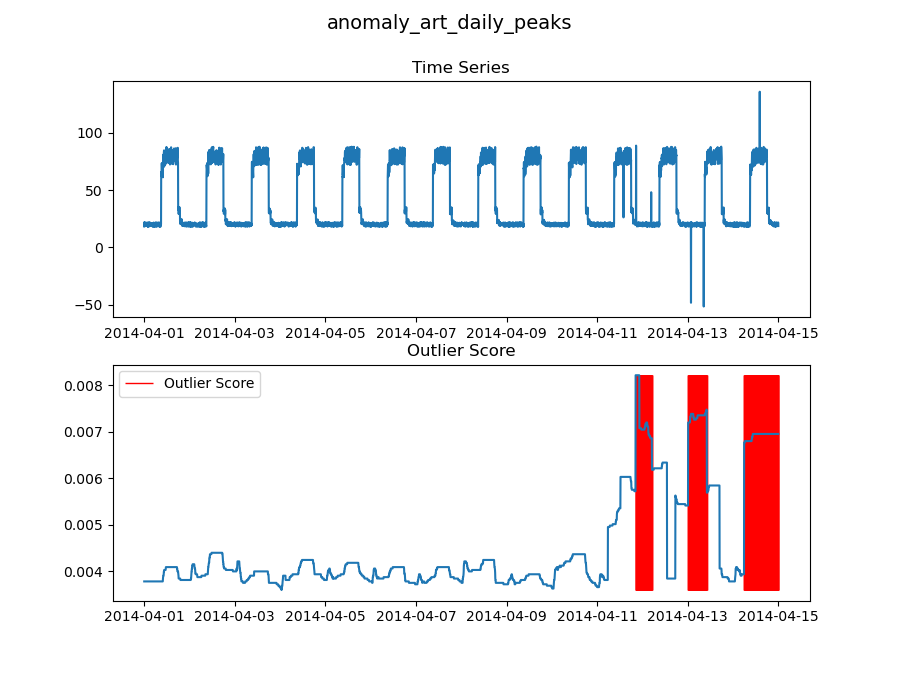
\includegraphics[width=0.5\textwidth]{fig/resultsPercolation/anomaly_art_daily_peaks}}
	\subfloat[Ausrei�er-Typ Frequenz�nderung\label{img:sequenceChangePerc}]{
		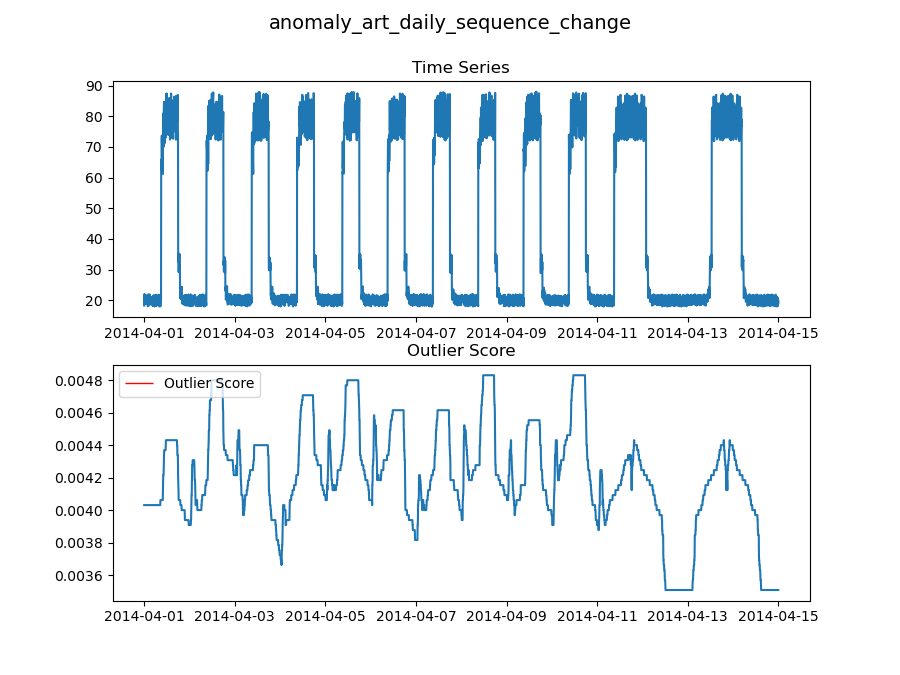
\includegraphics[width=0.5\textwidth]{fig/resultsPercolation/anomaly_art_daily_sequence_change}}
	\qquad
	\label{img:isomappictures1}
\end{figure}
\begin{figure}\ContinuedFloat
	\subfloat[Ausrei�er-Typ Kontinuierliche Zunahme der Amplitude\label{img:ampRisePerc}]{
		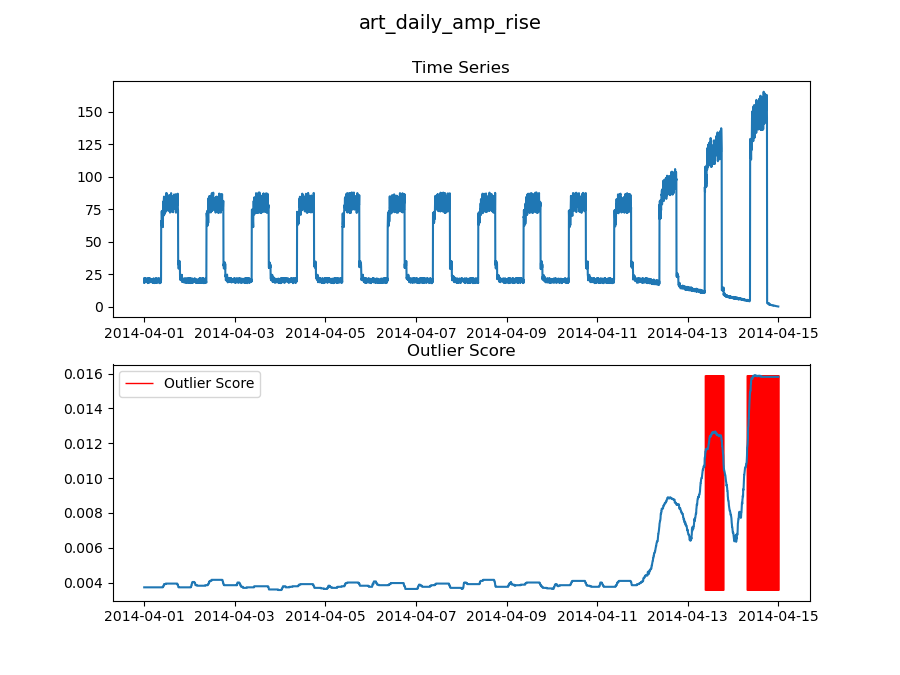
\includegraphics[width=0.5\textwidth]{fig/resultsPercolation/art_daily_amp_rise}}
	\subfloat[Ausrei�er-Typ Zyklus-Aussetzer\label{img:flatmiddlePerc}]{
		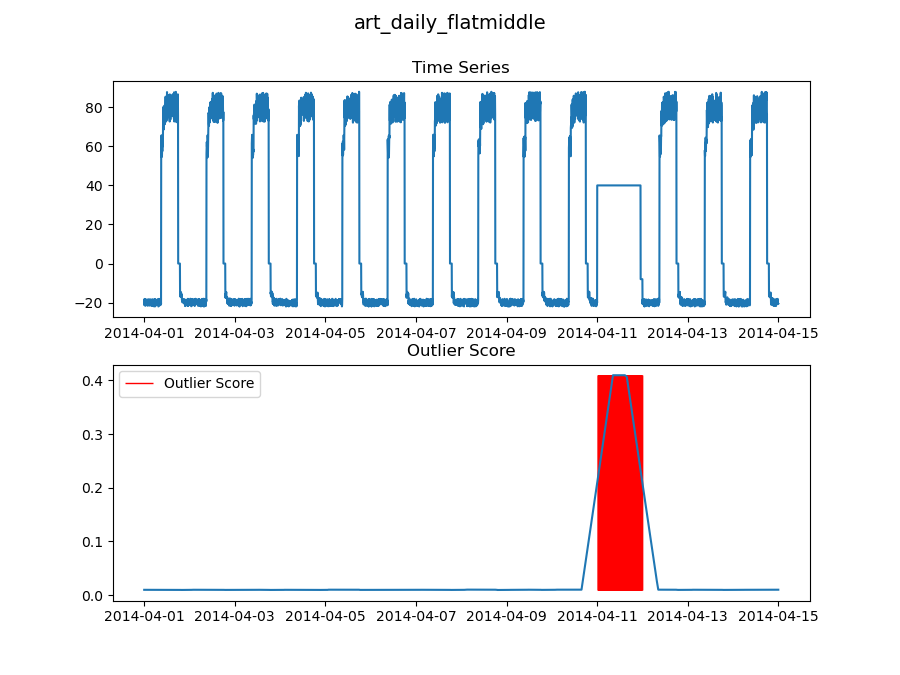
\includegraphics[width=0.5\textwidth]{fig/resultsPercolation/art_daily_flatmiddle}}
	\qquad
	\subfloat[Ausrei�er-Typ Zyklus mit geringerer Amplitude\label{img:jumpsdownPerc}]{
		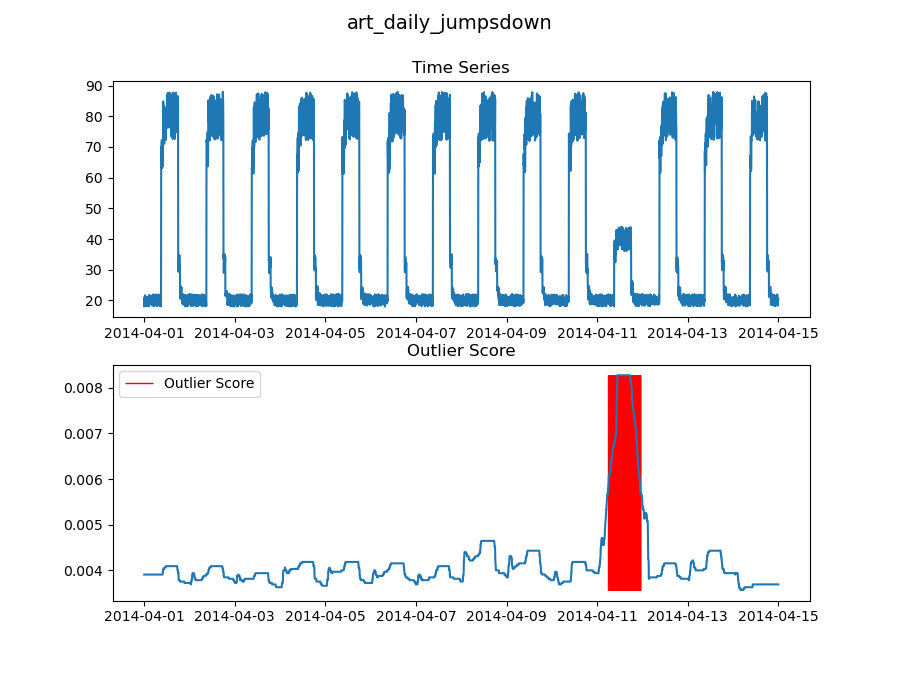
\includegraphics[width=0.5\textwidth]{fig/resultsPercolation/art_daily_jumpsdown}}
	\subfloat[Ausrei�er-Typ Zyklus mit h�herer Amplitude\label{img:jumpsupPerc}]{
		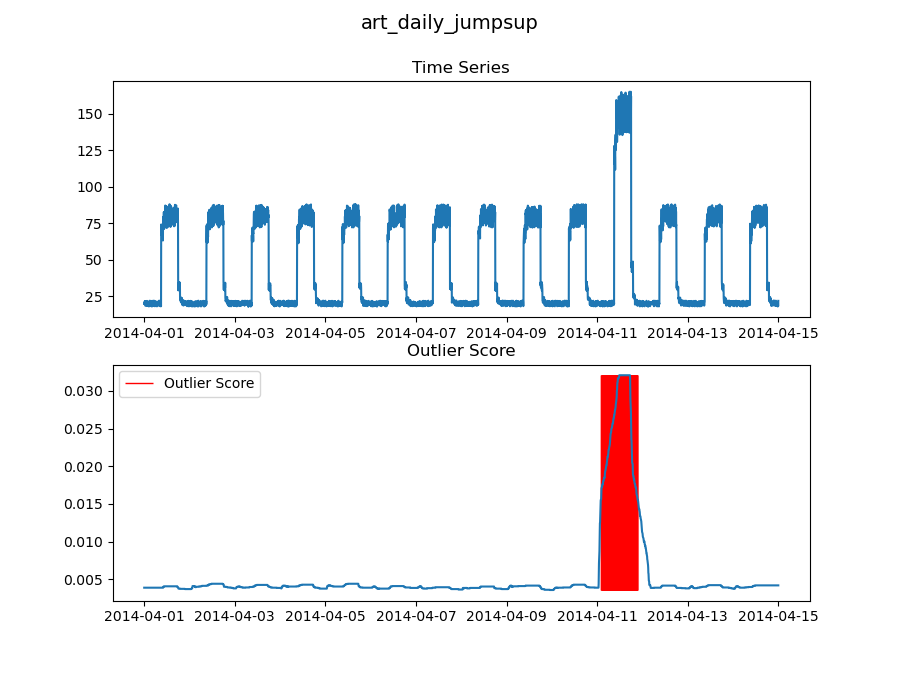
\includegraphics[width=0.5\textwidth]{fig/resultsPercolation/art_daily_jumpsup}}
	\qquad
	\subfloat[Ausrei�er-Typ Signal-Aussetzer\label{img:nojumpPerc}]{
		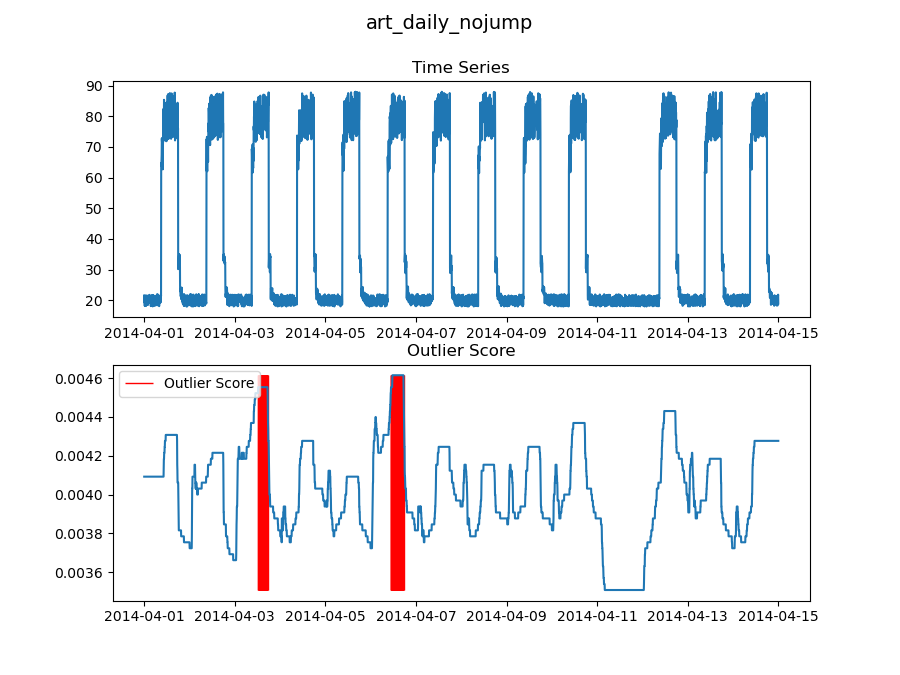
\includegraphics[width=0.5\textwidth]{fig/resultsPercolation/art_daily_nojump}}
	\label{img:isomappictures2}
\end{figure}


\newpage
